\documentclass[12pt,twoside]{extarticle}
\usepackage{extsizes}
\usepackage[paperheight=37.5cm,paperwidth=31.75cm, top=3.875cm,bottom=5.425cm,right=4.65cm,left=3.1cm]{geometry}
\usepackage[export]{adjustbox}
\usepackage{amsmath}
\usepackage{amsthm}
\usepackage{graphicx}
\usepackage{xcolor}
\usepackage{hyperref}
\usepackage{booktabs}
\usepackage{unicode-math}
%\unimathsetup{math-style=ISO, partial=upright, nabla=upright}
\setmainfont[Numbers=Tabular]{ScalaOT}
\setmathfont{Stix2Math.otf}
\setmathfont[range=it]{ScalaOT-Italic}
\setmathfont[range=\mathup/{num},Numbers={Tabular,Lining}]{ScalaOT}
%\setmathfont[range={"0030-"0039}]{ScalaOT}
\setmathfont[range=\mathup/{greek,Greek}]{Alegreya-Regular.otf}
\setmathfont[range=\mathit/{greek,Greek}]{Alegreya-Regular.otf}
\setmathfont[range={"002C}]{ScalaOT}
\setmathfont[range="002A]{ScalaOT}
\setmathfont[range={"222B},Scale=1.15]{LIBERTINUSMATH-REGULAR.otf}
\setmonofont[Scale=MatchUppercase]{NEXUSTYPEWRITERTF-REGULAR.otf}
\setsansfont[Numbers=Tabular]{SCALASANSPRO-REGULAR.otf}
\newfontfamily\myfontA[Numbers={Tabular,OldStyle}]{BEMBOBOOKMTSTD-REGULAR.otf}
\newfontfamily\myfontB[Numbers={Tabular,OldStyle}]{SCALASANSPRO-ITALIC.otf}
\newfontface\myfontC[]{AlegreyaSans-Regular.otf}
\definecolor{myblue}{RGB}{11, 79, 160}
\setlength{\footskip}{70pt}

\usepackage{listings} %For code in appendix
\lstset
{ %Formatting for code in appendix
    language=R,
    basicstyle=\footnotesize,
    numbers=left,
    stepnumber=1,
    showstringspaces=false,
    tabsize=1,
    breaklines=true,
    breakatwhitespace=false,
}

\begin{document}
\noindent 
 \begin{minipage}[t]{0.5\textwidth}
This seems like a pretty famous graph\footnotemark.  Let's try to draw it.
\end{minipage}\hfill
\footnotetext{\textsf{Credited to:  Tufte, Edward R. }\myfontB{The Visual Display of Quantitative Information}\textsf{.  But it looks like an attempt at a corrected version, because it differs from the one in the book.  I downloaded it from }\texttt{\url{https://www.edwardtufte.com/bboard/q-and-a-fetch-msg?msg_id=0003nk}}\textsf{ on May 12, 2019.}}
\adjustbox{valign=t}{\begin{minipage}[]{1\textwidth}
\vspace{2em} \raggedleft 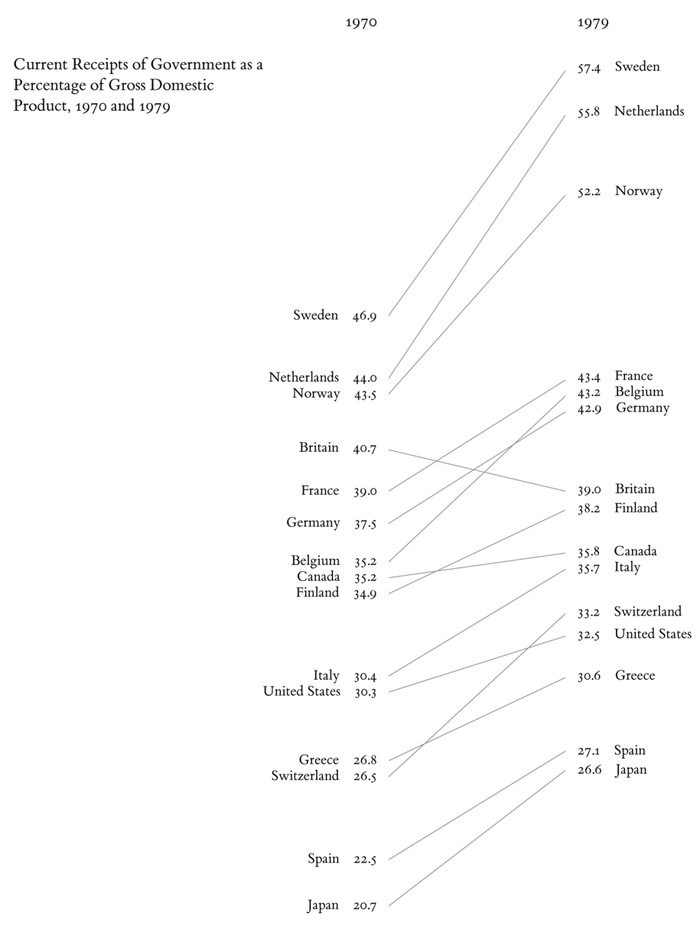
\includegraphics[]{TufteOrig.png}
\end{minipage}}%
\newpage
\noindent
\adjustbox{valign=t}{\begin{minipage}[8cm]{.53\textwidth}
\section{Drawing the Slopegraph}
Given two labeled columns of numbers, we begin by drawing on the usual Cartesian plane.  Each label's line is derived from two points, ($x_1$, $c_1$) and ($x_2$, $c_2$).  $x_1$ is the value from Column 1, $x_2$ is the value from Column 2.  $c_1$ and $c_2$ are the same for each line.  $c_2-c_1$ will determine the width of the final graph.  It can be changed by the constructor to adjust the aspect ratio.  The plane is rotated clockwise $90$° and flipped and a second set of labels is added.
The parameter $c_2-c_1$ now determines the $x$-axis.  We only need to ensure consistent spacing on the new $y$-axis to produce accurate slopes.  
\end{minipage}}%
\hfill
\adjustbox{valign=t}{\begin{minipage}[12cm]{0.42\textwidth}
\centering
\vspace{1em}
\begin{myfontA}
\bgroup
\def\arraystretch{1.25}%
\begin{tabular*}{7.5cm}%
{@{\extracolsep{\fill}}lrr@{}} \toprule
Country & 1970 & 1979 \\ \midrule
Sweden & 46.9 & 57.4 \\ 
Netherlands & 44.0 & 55.8 \\ 
Norway & 43.5 & 52.2 \\ 
Britain & 40.7 & 39.0 \\ 
France & 39.0 & 43.4 \\ 
Germany & 37.5 & 42.9 \\ 
Belgium & 35.2 & 43.2 \\ 
Canada & 35.2 & 35.8 \\ 
Finland & 34.9 & 38.2 \\ 
Italy & 30.4 & 35.7 \\
United States & 30.3 & 32.5 \\ 
Greece & 26.8 & 30.6 \\ 
Switzerland & 26.5 & 33.2 \\ 
Spain & 22.5 & 27.1 \\ 
Japan & 20.7 & 26.6 \\  \bottomrule
\end{tabular*}
\egroup
\end{myfontA}
\end{minipage}}
\adjustbox{valign=t}{\begin{minipage}[]{1\textwidth}
\end{minipage}}%
\newpage
\adjustbox{valign=t}{\begin{minipage}[28.2cm]{0.53\textwidth}
\end{minipage}}%
\hfill
\adjustbox{valign=t}{\begin{minipage}[t]{0.42\textwidth}
\section{ A First Attempt}
We'll plot using D3.js.  Tufte’s graph seems to be dropping $\approx$$24$ pixels for every $1$ percentage point in GDP, so that’s what we’ll use for our \textbf{\emph{drop coefficient}}.  We put the top point, Sweden[57.4], at position $0$, and every other point's position is determined by its distance from $57.4$ times $24$.  E.g., for Norway:  
\begin{gather}
y_1 = (57.4-43.5)\cdot 24=333.6 \\
y_2 = (57.4-52.2)\cdot24 =124.8
\end{gather}
Higher $y$-values move us further down the page because D3.js’s $y$-axis is upside-down.  In general, the drop coefficient is chosen to translate the scale of the data into something that fits on a screen.  In this case, the maximum element is $57.4$, the minimum is $20.7$, the difference is $57.4-20.7=36.7$.  If we let $1$ unit of the data equal $24$ pixels, our graph will be a little over $36.7 \cdot 24 \approx 881$ pixels long, which should be okay for a typical screen.  If the difference between the maximum and minimum of the data were more than $1000$, a drop coefficient $<1$ would probably be appropriate.\par
\vspace{1em}
The result is shown to the left.  Obviously, some points are too close together to get proper spacing for their labels.  There may be many ways to fix these crashed labels, and what's best will depend upon the situation.  Another approach would be constrained optimization.
\end{minipage}}
\newpage 
\noindent
\adjustbox{valign=c}{\begin{minipage}[t]{0.53\textwidth}
\section{Optimization}
We make the following assignments:
\begin{align*}
	&\left \{x_{1,j},... ,x_{n,j} \right \} &:=  \quad&\text{The numbers in column } j \text{ for } j=1,2 \\
	&\left \{y_{1,j},... ,y_{n,j} \right \} &:= \quad&\text{The vertical coordinates of the } x_{ij} \text{ at the beginning of the optimization.}\\
	&\left \{z_{1,j},... ,z_{n,j} \right \} &:= \quad&\text{The ideal placements of the } x_{ij} \text{ (if there were no concerns about crashed labels)} \\
	&\left \{\hat{y}_{1,j},... ,\hat{y}_{n,j} \right \} &:= \quad&\text{The fitted placements of the }x_{ij}
\end{align*}

The function to be optimized is the sum of squared distances between the points and their ideal placements.  The \textbf{objective function} is:

\begin{equation}
\sum_{j=1}^{2}\sum_{i=1}^{n}(z_{ij}-\hat{y}_{ij})^2
\end{equation}

The first constraint keeps the drop coefficients the same, within some tolerance.  Let  {\myfontC є} be some small number $>0$.  Let $k$ \text{ be the index of the set } $\left \{i \mid x_{i,1}-x_{i,2} \neq 0 \right \}$.  \textbf{Constraint 1:}

\begin{align*}
-\text{\myfontC є} \leq \frac{\hat{y}_{k,1}-\hat{y}_{k,2}}{x_{k,1}-x_{k,2}}\ - \frac{\hat{y}_{k+1,1}-\hat{y}_{k+1,2}}{x_{k+1,1}-x_{k+1,2}}\ &\leq \text{\myfontC є} \quad &\text{for } 1 < k < \lvert k \rvert \\
\hat{y}_{i,1}-\hat{y}_{i,2} &=0 \quad &\text{for } i \text{ such that } x_{i,1}-x_{i,2} = 0
\end{align*}

\textbf{Constraint 2} will make sure that the points stay in order, and that the minimum distance between them is $\zeta$ pixels, where $\zeta$ is chosen to provide the appropriate line spacing (I'm using $\zeta=16$ for an $11.5$ pt. font).

\begin{gather}
y_{1,j} - y_{1,i} \geq \zeta \quad \text{ for all }i,j \text{ s.t. }y_{1,j}^\ast > y_{1,i}^* \\
y_{2,j} - y_{2,i} \geq \zeta \quad \text{ for all }i,j \text{ s.t. }y_{2,j}^* > y_{2,i}^\text{*}
\end{gather}

Besides the first and last, every number in a column is sandwiched in between two other numbers.  We can make a constraint that puts the label closer to whichever number is closer.  E.g., we can place Germany[37.5] closer to France[39.0] than to Belgium[35.2], since $39.0-37.5 < 37.5-35.2$.  \textbf{Constraint 3:}

\begin{gather}
\text{for }i \text{ s.t. }\min(y_1) < y_{1,i}^* < \max(y_1) \\
\text{Let } y_{1,l} = \max(y_{1,j}^*:x_{1,j} < x_{1,i}), \\
y_{1,u} = \min(y_{1,j}^*:x_{1,j} > x_{1,i})\\
\text{if }x_{1,i}-x_l > x_u-x_i, \quad 2y_i-y_u-y_l > 0
\end{gather}

\textbf{Constraint 4} is the same as Constraint 3, except that it applies to Column 2. 


Other constraints could be added, but they'd reduce the number of potential solutions.  I wasn't able to get a graph on a scale close to Tufte's using all four constraints.  My graph is drawn under Constraints 1, 2, and 4. 
On my graph, it would be impossible to get Finland[38.2] as close to Britain[39.0] as Tufte has it.  Preserving the slope requires us to move both points the same distance, in the same direction, whenever we want to make an adjustment.  Moving Finland[38.2] up… 
Some lines are identical or nearly so, others are way off.  I know that my slopes are correct because there’s a check at the end of my code.
\end{minipage}}
\newpage
\begin{minipage}[]{0.42\textwidth}
\section{Comparison}
\textcolor{myblue}{My graph}, side-by-side with Tufte's:  The Sweden[57.4]'s are aligned as perfectly as I could get them.  The positionings of some points are close, but others are far off...
\end{minipage}%
\hfill
\vspace{1.5em}
\newpage
\newpage
\end{document}
